\subsection{Fundamental Group of a Quotient}

\subsubsection*{The Setup}

Here we give an example of a manifold \(N\) and a sub-manifold \(M\) embedded in \(N\) such that
the fundamental group of the quotient, \(\pi_1(N / M)\) is NOT homomorphic to \(\pi_1(N) / \pi_1(M)\).
In particular, it matters how \(M\) is embedded in \(N\). 

For our example, \(N = T^3\), the 3-torus which can be viewed as the fundamental cube \(\{0 \leq x, y, z\leq 1\}\)
under the identifications
\begin{equation}
\begin{cases}
(x, y, z) \equiv (x + 1, y, z), \\
(x, y, z) \equiv (x, y + 1, z), \\
(x, y, z) \equiv (x, y, z + 1).
\end{cases}
\end{equation} 
The effect is to identify opposite faces.

We will embed \(M = S^1\) in a nontrivial way; we let \(M\) wrap around twice in the z-direction without crossing
itself. See the figure below.
\begin{figure}[h]
\centering
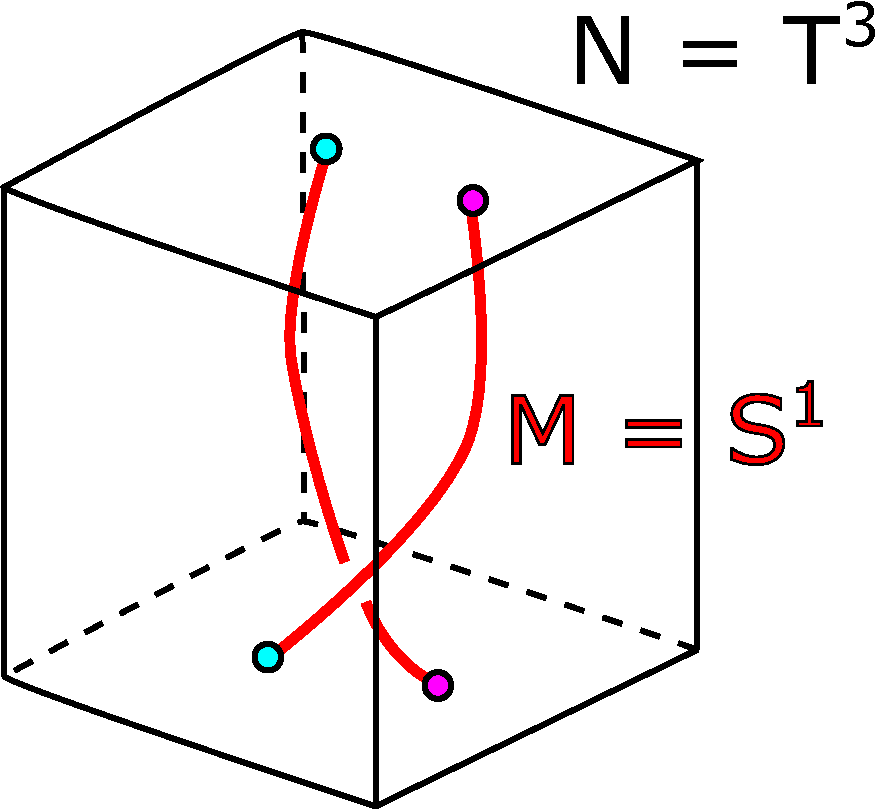
\includegraphics[width=2.5in]{Topology/FundamentalGroupQuotient/embedding.pdf}
\end{figure} 

\subsubsection*{The Problem}

Compute the fundamental group of the quotient \(N / M\) as described above.

\subsubsection*{The Solution}

To compute \(\pi_1(N / M)\), we will use the Seifert-van Kampen theorem. We cover \(N\) by two open sets \(U_1\)
\(U_2\). The first open set \(U_1\) consists of everything in \(N\) outside a closed torus enclosing \(M\). The
open set \(U_2\) is simply an open torus containing \(M\). Their intersection is simply an open solid annular torus.
See the figure below.  
\begin{figure}[h]
\centering
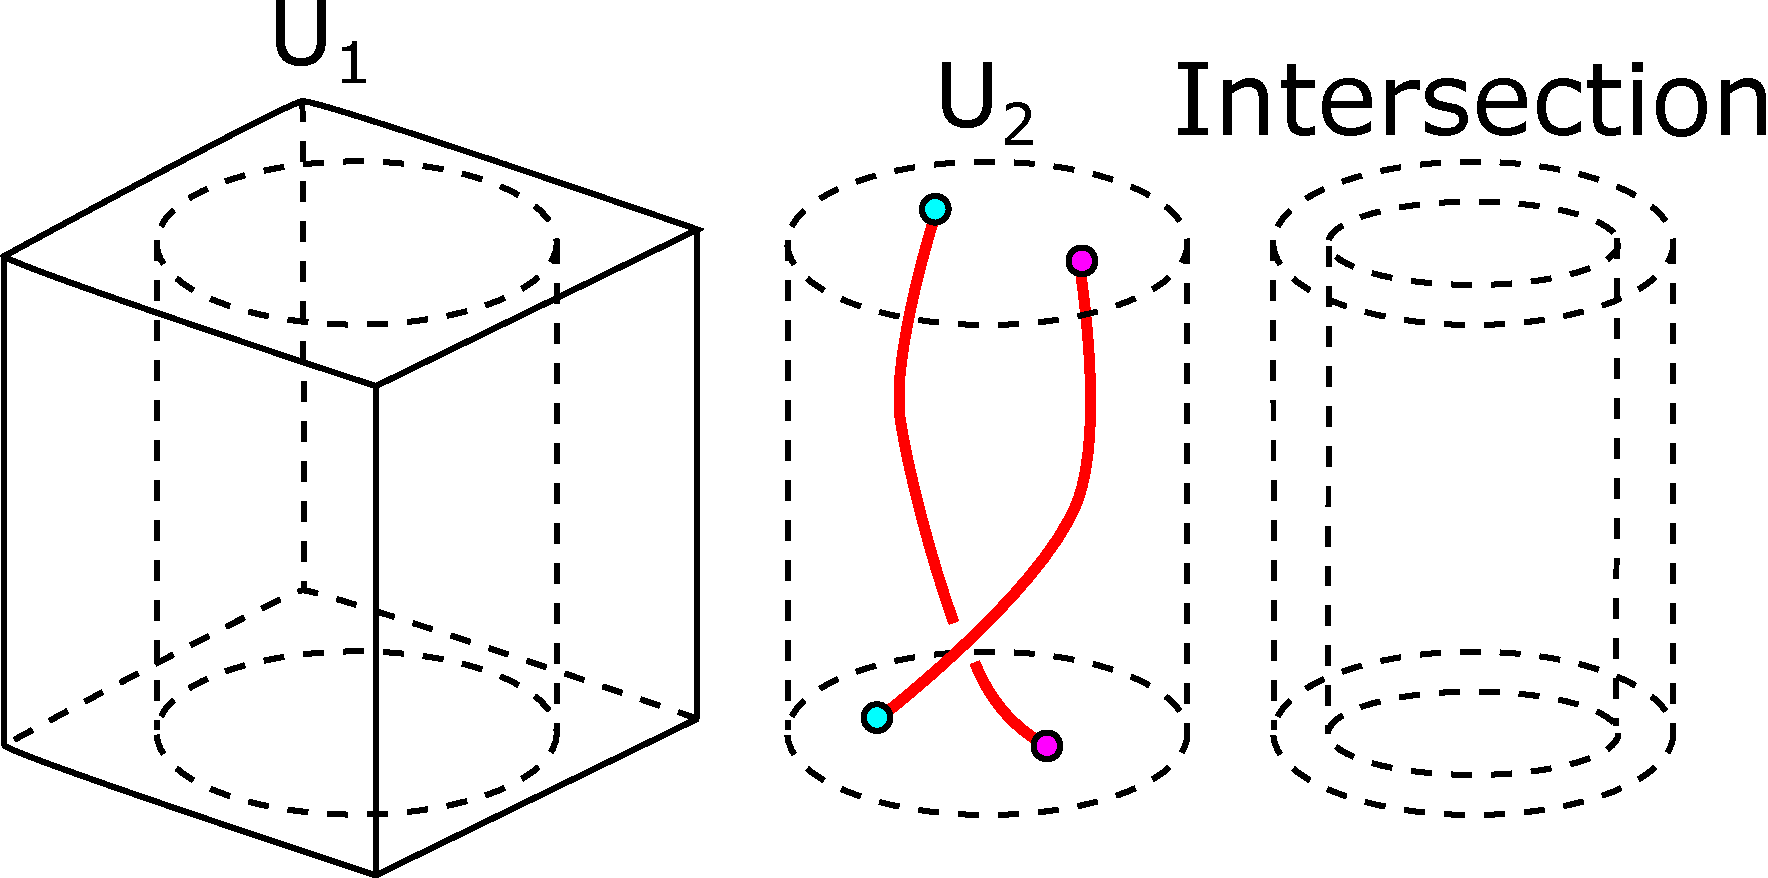
\includegraphics[width = 4.5in]{Topology/FundamentalGroupQuotient/split.pdf}
\end{figure}

Let us first consider how to compute fundamental group for the neighborhood containing \(M\), \(\pi_1(U_2)\). We
see that \(U_2\) deformation retracts onto a mobius strip whose edges are \(M\); for the quotient, this is a
mobius strip with its edges identified as one single point, which we will call \(P\). See the figure below.

\begin{figure}[h]
\centering
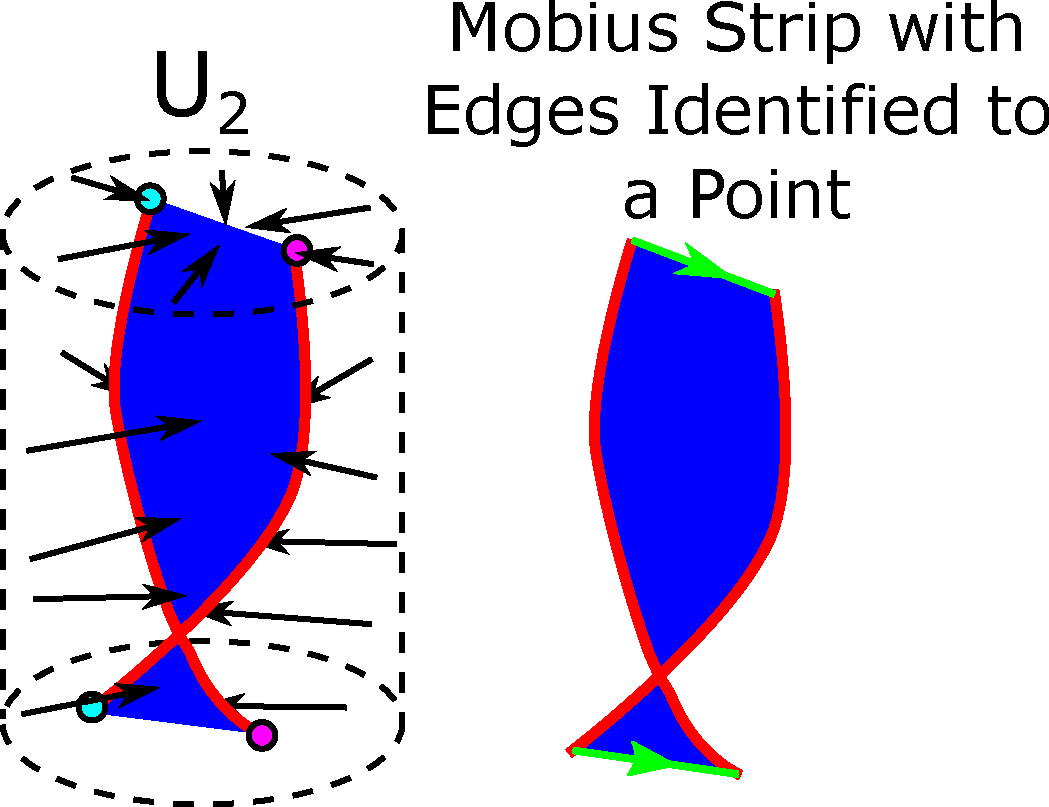
\includegraphics[width = 3.5in]{Topology/FundamentalGroupQuotient/deformationRetract.pdf}
\end{figure}

We need to compute \(\pi_1(P)\). For this, we can again apply Seifer-van Kampen. First, consider the meridian 
curve \(m\) that runs along the waist of the 
mobius strip, see the figure below. 

\begin{figure}[h]
\centering
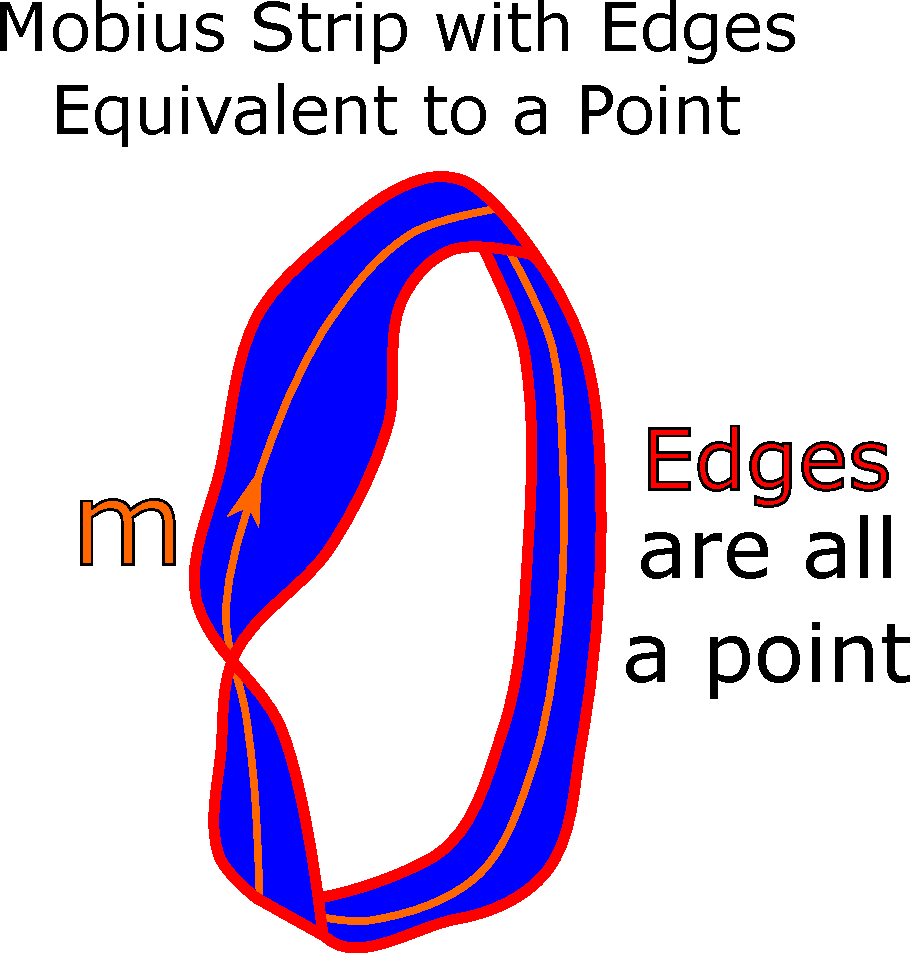
\includegraphics[width=2in]{Topology/FundamentalGroupQuotient/mobius.pdf}
\end{figure}
Let \(V_1\) be a neighborhood of
the meridian curve \(m\). Then let \(V_2\) be a neighborhood of 
the edges such that \(V_1\) and \(V_2\) cover \(P\). Note that the twist in the Mobius strip gives us that
\(V_1 \cap V_2\) is connected.

Now, \(V_2\) deformation retracts to the edges of the Mobius strip, which for \(P\) is just a single point.
Therefore, \(V_2\) is simply connected, i.e. \(\pi_1(V_2) = \{1\}\). Next, we note that \(V_1\) deformation
retracts to the meridian \(m\), which is an \(S^1\). Therefore, \(\pi_1(V_1)\) is just the free group 
generated by \(m\), i.e. \(\pi_1(V_1) = (m)\)..

Next, observe that \(V_1 \cap V_2\) is in fact a cylindrical strip; therefore \(\pi_1(V_1 \cap V_2)\) is generated
by the loop going around it. Now we see that such a loop covers \(m\) twice; so being a little loose with
notation, \(\pi_1(V_1 \cap V_2) = (m^2)\).

Therefore, by Seifert-van Kampen, we have that \(\pi_1(U_2) = \pi_1(P) = (m) / (m^2) = \mathbb Z_2\).

Next, consider \(U_1\). We see that \(U_1\) deformation retracts onto \((S^1 \vee S^1) \times S^1\). We
denote the generators by \(x, y\) and \(z\); each denotes its usual direction. See the figure below.
So \(\pi_1(U_1) = ((x) \star (y))\times (z)\).

\begin{figure}[h]
\centering
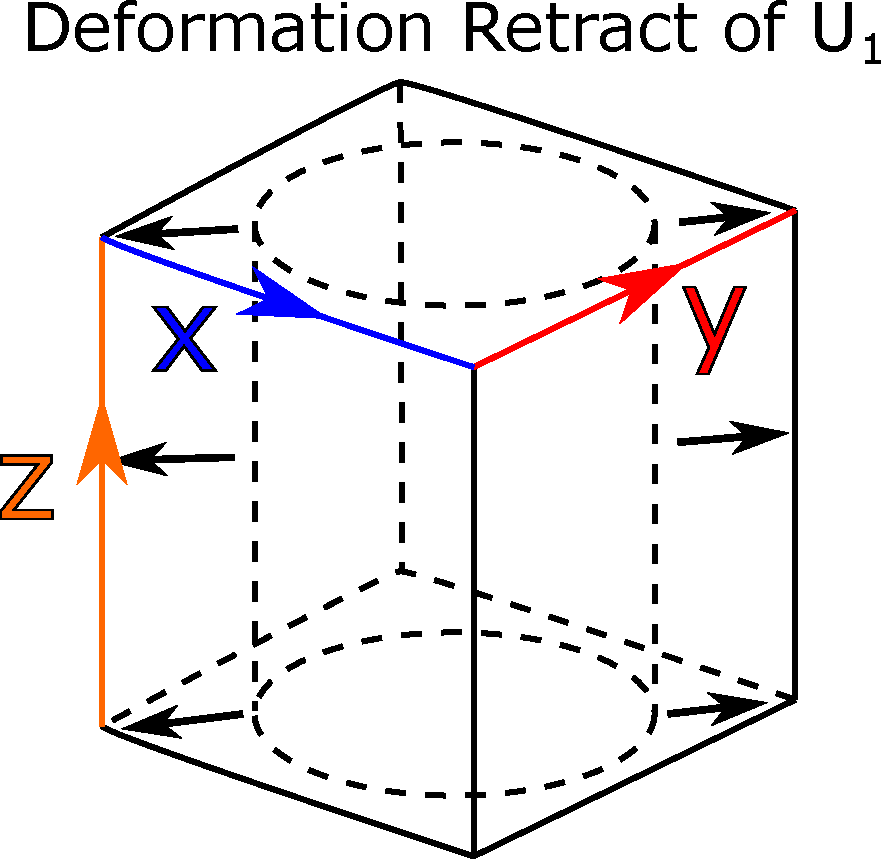
\includegraphics[width = 2.5in]{Topology/FundamentalGroupQuotient/deformationRetract2.pdf}
\end{figure} 

Finally, we need to consider \(U_1 \cap U_2\). It is pretty clear that \(\pi_1(U_1 \cap U_2)\) is generated by
a horizontal counter-clockwise circle and a vertical upwards loop. Also, it is clear that the horizontal 
circle is equivalent to \(xyx^{-1}y^{-1}\) inside \(U_1\), and the upward loop is equivalent to \(z\) inside
\(U_1\). We need to consider their equivalents inside \(U_2\). 

It isn't hard to see that the vertical loop retracts onto the meridian \(m\); however, note that it doesn't
retract onto the edges. The horizontal circle retracts onto a loop that double backs on itself, and so up to
homotopy is trivial. See the figure below. 

\begin{figure}[H]
\centering
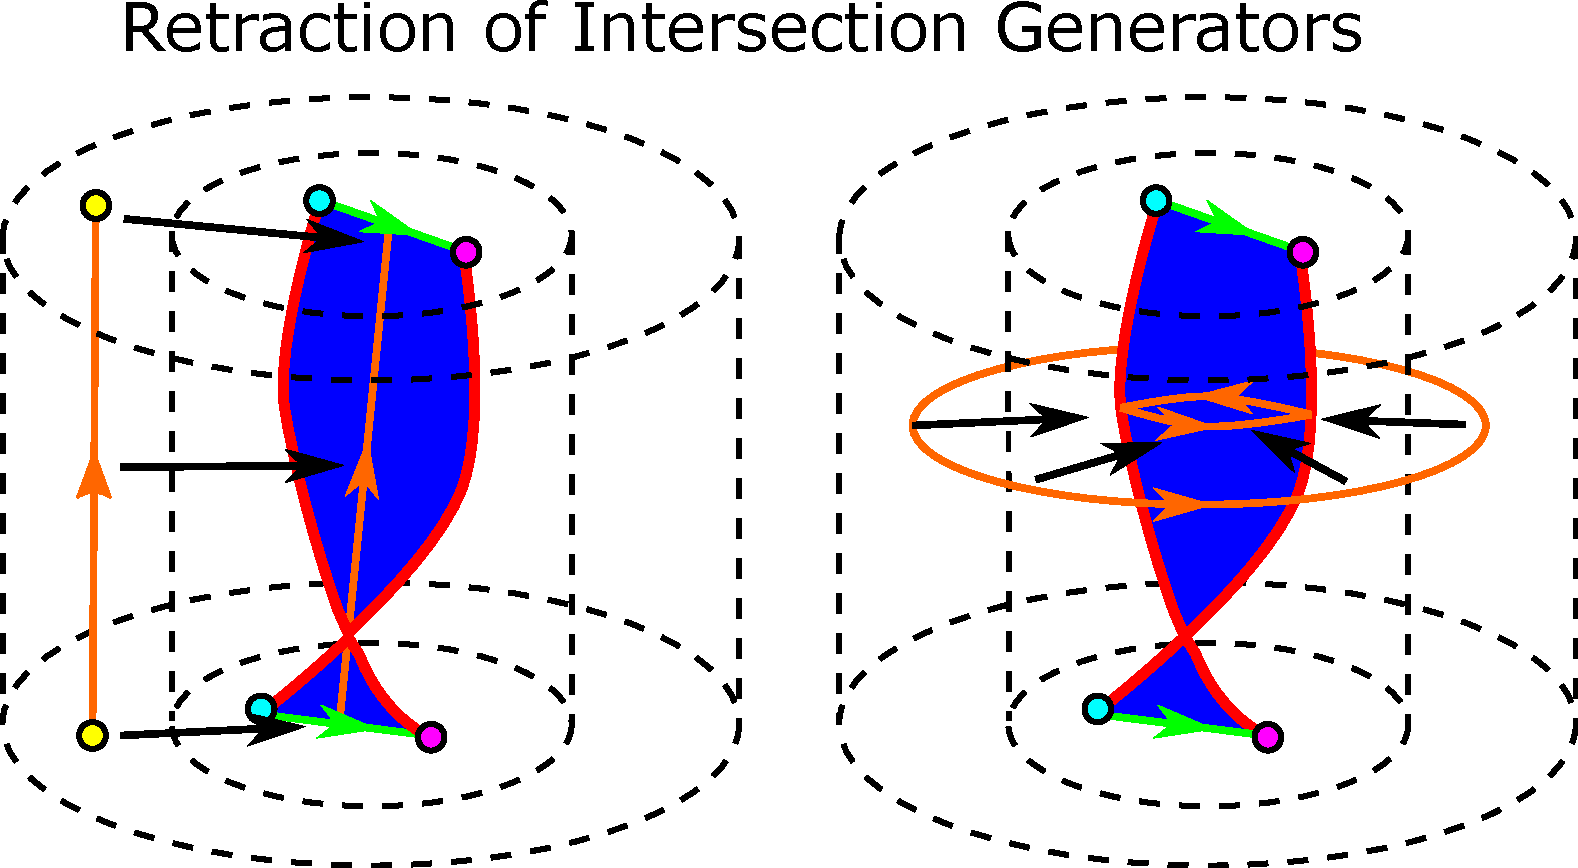
\includegraphics[width = 3.5in]{Topology/FundamentalGroupQuotient/intersection.pdf}
\end{figure}

So we see that the normal group generated by \(i_\star(U_1) i_\star(U_2)^{-1}\) is generated by
\(xyx^{-1}y^{-1}\) and \(zm^{-1}\). By Seifer-van Kampen, we have
\begin{align}
\pi_1(N / M) & = \frac{ [((x)\star (y))\times (z)] \star [(m) / (m^2)]} {(xyx^{-1}y^{-1}, zm^{-1}) }, \\
    & = \frac{(x)\times(y)\times(z)}{(z^2)}, \\
    & = \mathbb Z \times \mathbb Z \times \mathbb Z_2. 
\end{align}
